\documentclass{beamer}
\usepackage[final]{listings}
\usetheme{Madrid}
\usecolortheme{beaver}
\usefonttheme{professionalfonts}
\setbeamertemplate{footline}[page number]{}
\setbeamertemplate{navigation symbols}{}
\definecolor{burgundy}{rgb}{0.82, 0.1, 0.26}

\begin{document}
	
\title
{
	\texttt{bencherl}: A scalability benchmark suite for Erlang/OTP
}

\author
{
	Stavros Aronis\inst{1} \and
	Nikolaos Papaspyrou\inst{2} \and
	\textcolor{burgundy}{Katerina Roukounaki}\inst{2} \and
	Konstantinos Sagonas\inst{1,2} \and
	Yiannis Tsiouris\inst{2} \and
	Ioannis Venetis\inst{2}
}

\institute
{
	\inst{1}%
	Department of Information Technology, Uppsala University, Sweden
	\and
	\inst{2}%
	School of Electrical and Computer Engineering, National Technical University of Athens, Greece
}

\date
{Erlang Workshop 2012, Copenhagen}

\begin{frame}
	\titlepage
\end{frame}

\begin{frame}{Motivation}
	\begin{block}{Frustrated Erlang programmer}
		I thought my Erlang program was {\bf 100\% parallelizable}, but when I made it parallel and ran it on a machine with {\bf N CPU cores}, I got a {\bf speedup} that was {\bf much lower than N}. Why?
	\end{block}
\end{frame}

\begin{frame}[t]{\texttt{bencherl}}
	\begin{itemize}
		\item Serves both as a \textcolor{burgundy}{tool to run and analyze benchmarks} and as an \textcolor{burgundy}{enhanceable benchmark repository}
		\item Focuses on \textcolor{burgundy}{scalability}, rather than on throughput or latency
		\item Examines how the following \textcolor{burgundy}{factors} influence the scalability of Erlang applications
			\begin{itemize}
				\item Number of Erlang nodes
				\item Number of CPU cores
				\item Number of schedulers
				\item Erlang/OTP release and flavor
				\item Command-line arguments to \texttt{erl}
			\end{itemize}
		\item Can be used to study the performance of any \textcolor{burgundy}{Erlang application}, as well as for the \textcolor{burgundy}{Erlang/OTP} itself
	\end{itemize}
\end{frame}

\begin{frame}[t]{Definitions}

	\vspace{5pt}
	{\bf Application}: The \textcolor{burgundy}{piece of software} whose execution behaviour we intend to measure and analyze.

    \vspace{5pt}
	{\bf Benchmark}: A specific \textcolor{burgundy}{use case} of the \textcolor{burgundy}{application} that includes setting up the environment, calling specific functions and using specific data.

    \vspace{5pt}
	{\bf Runtime environment}: A specific combination of values for the \textcolor{burgundy}{scalability factors}.
	\begin{itemize}
		\item E.g. 8 \textcolor{burgundy}{Erlang nodes} on a machine with 64 \textcolor{burgundy}{CPU cores} using 8 \textcolor{burgundy}{schedulers} on each node and running Erlang/OTP R15B02 \textcolor{burgundy}{release} with \textcolor{burgundy}{command-line arguments} "+sbt db" 
	\end{itemize}
\end{frame}

\begin{frame}[t]{Architecture}
	\begin{center}
		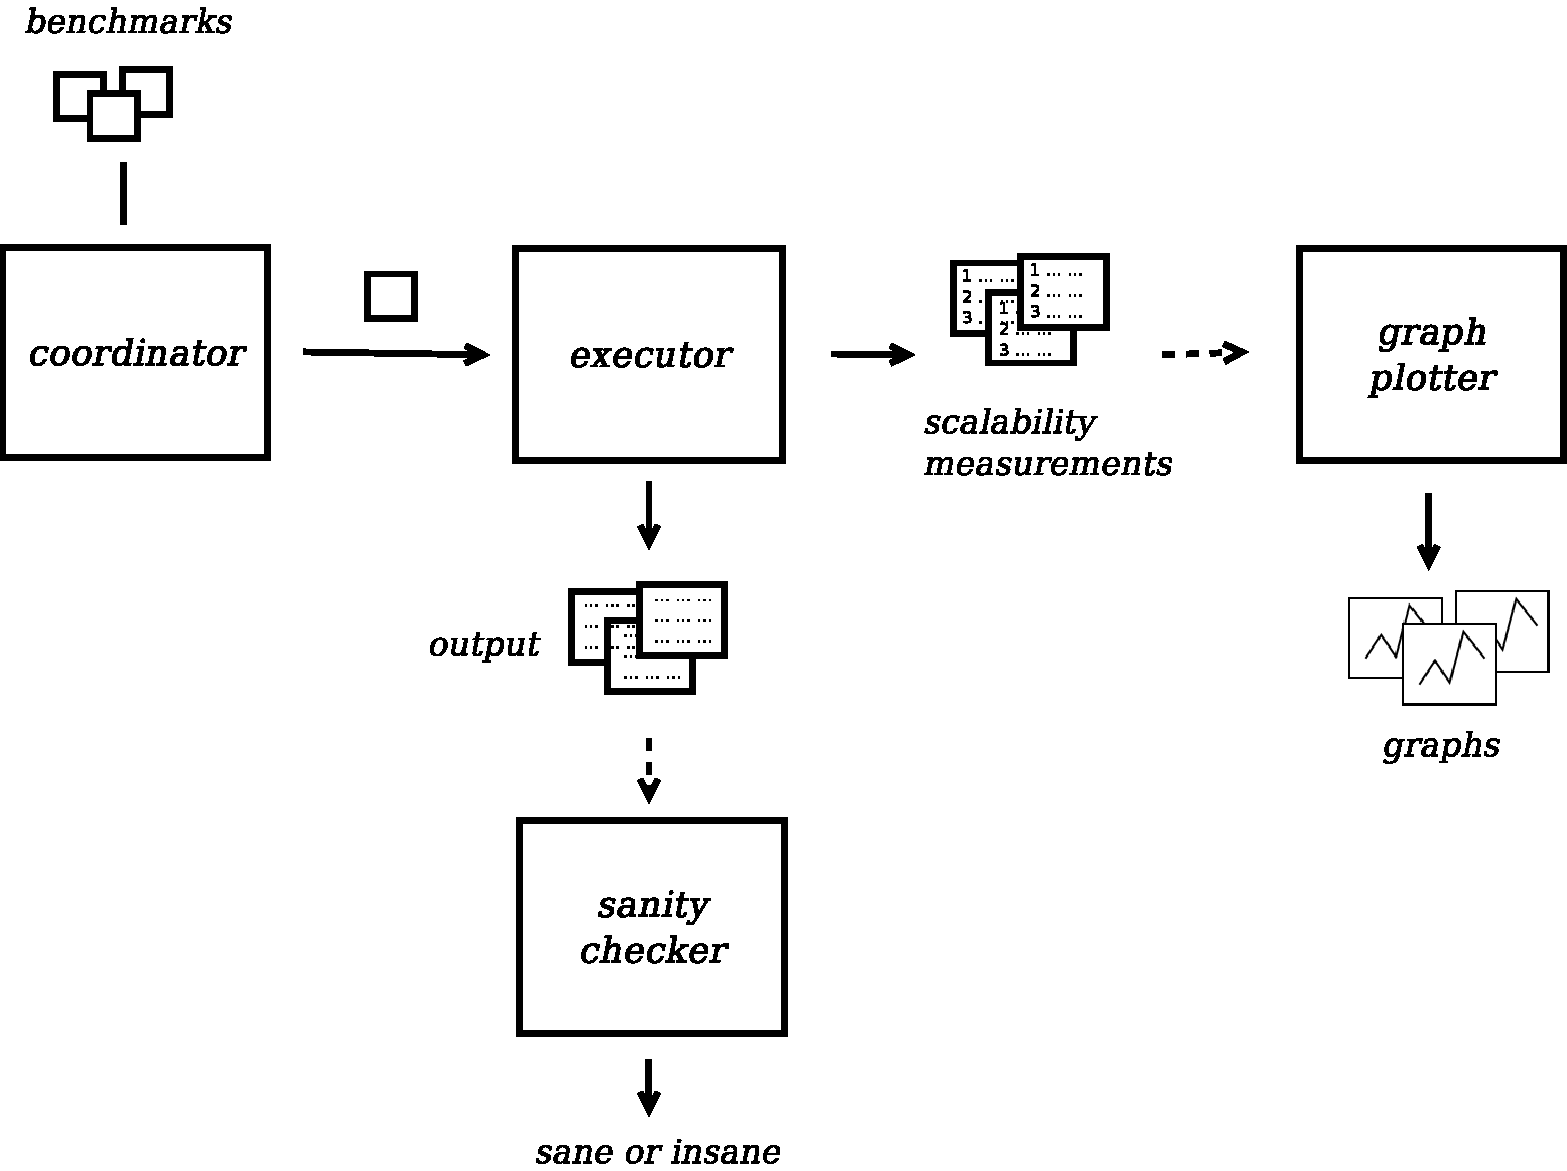
\includegraphics[width=0.8\linewidth]{figures/architecture.pdf}
	\end{center}
\end{frame}

\begin{frame}[t]{Coordinator}
	{\bf The module that coordinates everything during a \texttt{bencherl} run.}
	\begin{itemize}
		\item Determines the \textcolor{burgundy}{benchmarks} that should be executed
		\item Determines the \textcolor{burgundy}{runtime environments}, where each benchmark should be executed
		\item \textcolor{burgundy}{Sets up} each runtime environment before a benchmark is executed in it
		\item Prepares instruction files for the \textcolor{burgundy}{executor}
		\item Performs any \textcolor{burgundy}{benchmark-specific pre- and post-execution actions}
	\end{itemize}
\end{frame}

\begin{frame}[t]{Executor}
	{\bf The module that executes a particular benchmark in a particular runtime environment.}
	\begin{itemize}
		\item Receives detailed instructions from the \textcolor{burgundy}{executor} about what to do 
		\item \textcolor{burgundy}{Starts} any necessary Erlang slave nodes
		\item \textcolor{burgundy}{Executes} the benchmark in a new process
		\item \textcolor{burgundy}{Stops} the Erlang slave nodes it started
		\item Makes sure that the \textcolor{burgundy}{output} that the benchmark produced during its execution is written in an output file
		\item Makes sure that the \textcolor{burgundy}{measurements} that are collected during the execution of the benchmark are written in a measument file 
			\begin{itemize}
				\item Uses \texttt{erlang:now/0} and \texttt{timer:diff/2}
			\end{itemize}
	\end{itemize}
\end{frame}

\begin{frame}[t]{Sanity checker}
	{\bf The module that checks whether all executions of a particular benchmark produced the same output.}
    \begin{itemize}
		\item Runs \textcolor{burgundy}{after} a benchmark has executed in all desired runtime environments
		\item \textcolor{burgundy}{Examines} the output that the benchmark produced in all runtime environments
		\item Decides whether the benchmark was \textcolor{burgundy}{successfully executed} in all runtime environments
		\item Is based on the assumption that if a benchmark produces any output during its execution, then this output should be \textcolor{burgundy}{the same accross all runtime environments}, where the benchmark was executed
			\begin{itemize}
				\item Uses \texttt{diff}
			\end{itemize}
    \end{itemize}
\end{frame}

\begin{frame}[t]{Graph plotter}
	{\bf The module that plots scalability graps based on the collected measurements.}
    \begin{itemize}
		\item Runs \textcolor{burgundy}{after} a benchmark has executed in all desired runtime environments
		\item Processes the \textcolor{burgundy}{measurements} that were collected during the execution of the benchmark
		\item Plots a set of scalability graphs
			\begin{itemize}
				\item Uses \texttt{Gnuplot}
			\end{itemize}
    \end{itemize}
\end{frame}

\begin{frame}[t]{Scalability graphs}
	\begin{itemize}
		\item Both \textcolor{burgundy}{time} and \textcolor{burgundy}{speedup} graphs
		\item Graphs that show how benchmarks scale when executed with specific erl version and command-line arguments and with \textcolor{burgundy}{different number of schedulers (nodes)}
		\item Graphs that show how benchmarks scale when executed with specific erl version and with \textcolor{burgundy}{different number of schedulers (nodes) and runtime options}
		\item Graphs that show how benchmarks scale when executed with specific erl runtime options and with \textcolor{burgundy}{different number of schedulers (nodes) and erl versions}
	\end{itemize}
\end{frame}

\begin{frame}[t]{Benchmarks}
	\texttt{bencherl} comes with an initial collection of benchmarks.
    \vspace{10pt}
	\begin{columns}[t]
		\begin{column}{0.5\textwidth}
			\begin{center}
			\textcolor{burgundy}{synthetic}
			\begin{columns}
				\begin{column}{0.6\textwidth}
					\begin{itemize}
						\item[] \texttt{bang}
						\item[] \texttt{big}
						\item[] \texttt{ehb}
						\item[] \texttt{ets\_test}
						\item[] \texttt{genstress}
						\item[] \texttt{mbrot}
					\end{itemize}
				\end{column}
				\begin{column}{0.45\textwidth}
					\begin{itemize}
						\item[] \texttt{orbit\_int}
						\item[] \texttt{parallel}
						\item[] \texttt{pcmark}
						\item[] \texttt{ran}
						\item[] \texttt{serialmsg}
						\item[] \texttt{timer\_wheel}
					\end{itemize}
				\end{column}
			\end{columns}
			\end{center}	
		\end{column}
        \begin{column}{0.3\textwidth}
			\begin{center}	
			\textcolor{burgundy}{real-world}
			\begin{itemize}
				\item[] \texttt{dialyzer\_bench}
				\item[] \texttt{scalaris\_bench}
			\end{itemize}
			\end{center}
        \end{column}
	\end{columns}	
	\vspace{20pt}
	This collection can be \textcolor{burgundy}{enhanced} in two simple steps.
\end{frame}

\begin{frame}[t]{Step 1: Add in \texttt{bencherl} everything that the benchmark needs for its execution.}
	\begin{itemize}
		\item The sources of the \textcolor{burgundy}{Erlang application} that it benchmarks
			\begin{itemize}
				\item E.g. \texttt{dialyzer}
			\end{itemize}
		\item Any \textcolor{burgundy}{scripts} to run \textcolor{burgundy}{before} or \textcolor{burgundy}{after} its execution
            \begin{itemize}
                \item E.g. a script that starts \texttt{scalaris}
            \end{itemize}
		\item Any \textcolor{burgundy}{data} that it needs for its execution
            \begin{itemize}
                \item E.g. for \texttt{dialyzer\_bench} the BEAM files
            \end{itemize}
		\item Any specific \textcolor{burgundy}{configuration settings} that it requires
            \begin{itemize}
                \item E.g. a specific cookie that nodes should share
            \end{itemize}
	\end{itemize}
\end{frame}

\begin{frame}[fragile]{Step 2: Write the handler for the benchmark.}
	A \textcolor{burgundy}{benchmark handler} is a standard Erlang module that exports two functions.
	\vspace{10pt}

	\textcolor{burgundy}{\texttt{bench\_args}}: a function that returns the different argument sets that should be used for running a specific version of the benchmark

	\tiny
	\begin{verbatim}
bench_args(Vrsn, Conf) -> Args
  when
    Vrsn :: 'short' | 'intermediate' | 'long',
    Conf :: [{Key :: atom(), Val :: term()}, ...],
    Args :: [[term()]].
	\end{verbatim}
	\normalsize

	\textcolor{burgundy}{\texttt{run}}: a function that runs the benchmark on specific Erlang nodes, with specific arguments and configuration settings

	\tiny
    \begin{verbatim}
run(Args, Slaves, Conf) -> 'ok' | {'error', Reason}
  when
    Args   :: [term()],
    Slaves :: [node()],
    Conf   :: [{Key :: atom(), Val :: term()}, ...],
    Reason :: term().
	\end{verbatim}
	\normalsize

\end{frame}

\begin{frame}[fragile]{A benchmark handler example}

	\tiny
    \begin{verbatim}
-module(scalaris_bench).

-include_lib("kernel/include/inet.hrl").

-export([bench_args/2, run/3]).

bench_args(Version, Conf) ->
    {_,Cores} = lists:keyfind(number_of_cores, 1, Conf),
	[F1, F2, F3] = case Version of
		short -> [1, 1, 0.5];
		intermediate -> [1, 8, 0.5];
		long -> [1, 16, 0.5]
	end,
	[[T,I,V] || T <- [F1 * Cores], I <- [F2 * Cores], V <- [trunc(F3 * Cores)]].

run([T,I,V|_], _, _) ->
	{ok, N} = inet:gethostname(),
	{ok, #hostent{h_name=H}}=inet:gethostbyname(N),
	Node = "firstnode@" ++ H,
	rpc:block_call(list_to_atom(Node), api_vm, add_nodes, [V]),
	io:format("~p~n", [rpc:block_call(list_to_atom(Node), bench, quorum_read, [T,I])]),
	ok.
	\end{verbatim}
	\normalsize
\end{frame}

\begin{frame}{Experience \#1: Some benchmarks scale well.}
	\begin{center}
		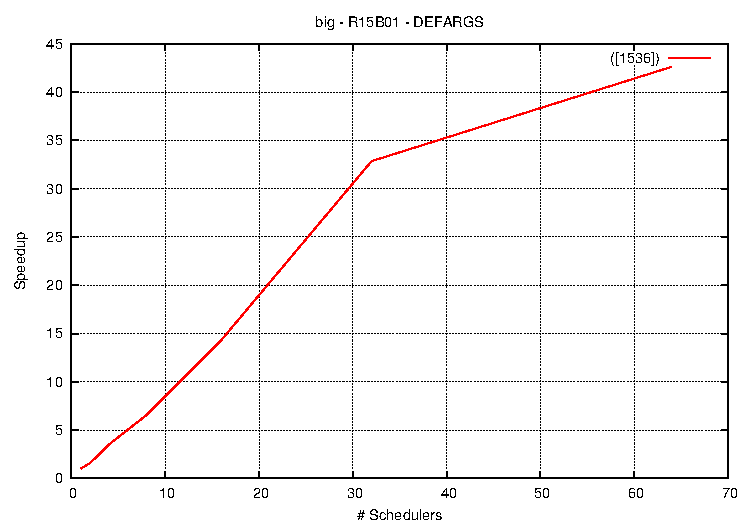
\includegraphics[width=0.8\linewidth]{figures/big-speedup-bulldozer.pdf}
	\end{center}
\end{frame}

\begin{frame}{Experience \#2: Some benchmarks scale do not scale as well on more than one nodes.}
    \begin{center}
        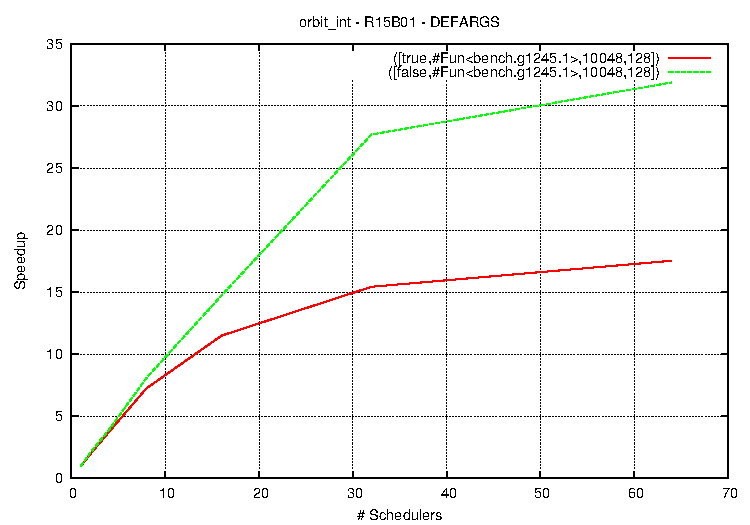
\includegraphics[width=0.45\linewidth]{figures/orbit_int_par-speedup-bulldozer.pdf}
        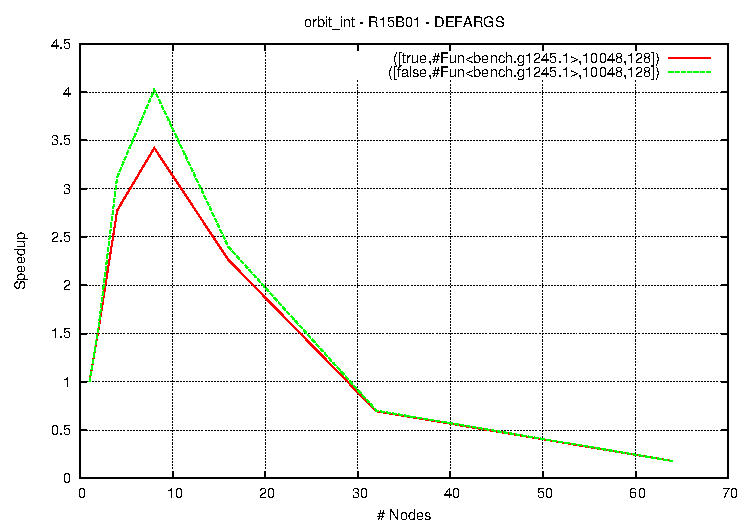
\includegraphics[width=0.45\linewidth]{figures/orbit_int_dist-speedup-bulldozer.pdf}
    \end{center}
\end{frame}

\begin{frame}{Experience \#3: Some benchmarks do not scale.}
    \begin{center}
        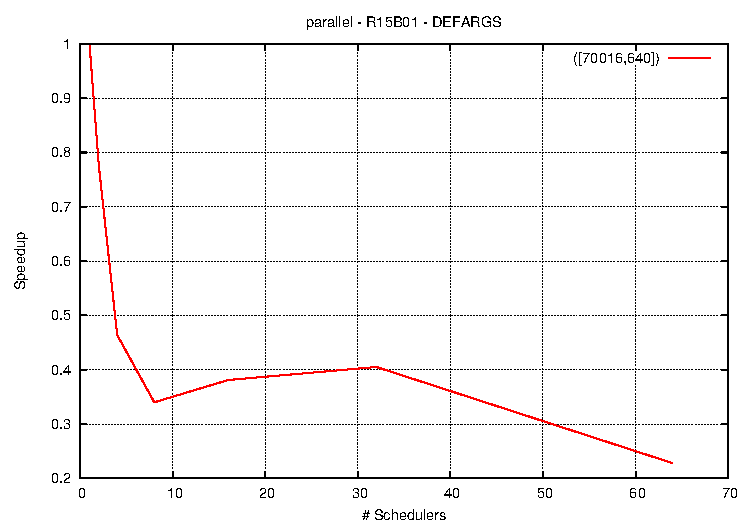
\includegraphics[width=0.8\linewidth]{figures/parallel-speedup-bulldozer.pdf}
    \end{center}
\end{frame}

\begin{frame}{Experience \#4: Some benchmarks scale better with specific runtime options.}
    \begin{center}
        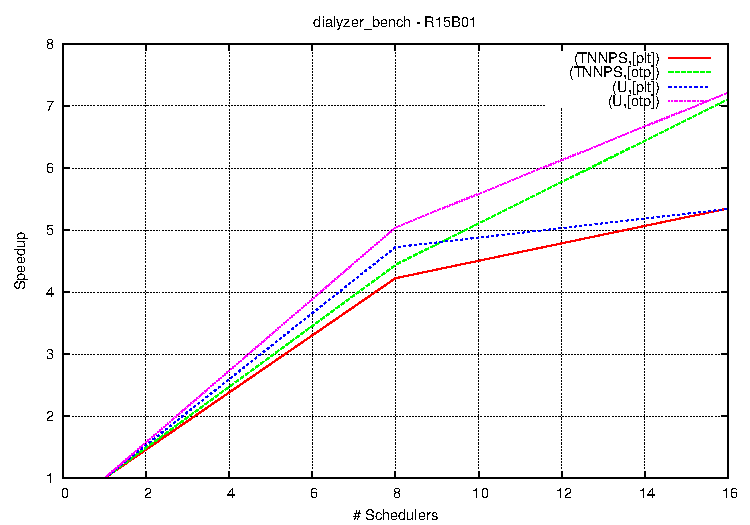
\includegraphics[width=0.8\linewidth]{figures/dialyzer_bench-speedup-bulldozer.pdf}
    \end{center}
\end{frame}

\begin{frame}{Experience \#5: Some benchmarks scale better with specific Erlang/OTP releases.}
    \begin{center}
        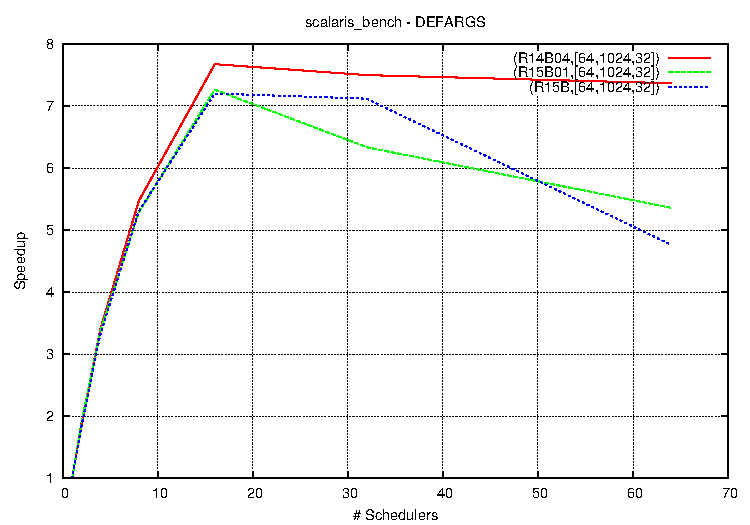
\includegraphics[width=0.8\linewidth]{figures/scalaris-speedup-bulldozer.pdf}
    \end{center}
\end{frame}

\begin{frame}[t]{Conclusions}
	\begin{itemize}
		\item \texttt{bencherl} is a publicly available, \textcolor{burgundy}{scalability} benchmark suite for Erlang/OTP
			\begin{itemize}
				\item \texttt{http://release.softlab.ntua.gr/bencherl}
			\end{itemize} 
		\item Examines how \textcolor{burgundy}{nodes}, \textcolor{burgundy}{cores}, \textcolor{burgundy}{schedulers}, \textcolor{burgundy}{Erlang/OTP versions} and \textcolor{burgundy}{\texttt{erl} command-line options} affect the scalability of Erlang applications
		\item Collects \textcolor{burgundy}{scalability measurements}
		\item Plots \textcolor{burgundy}{scalability graphs}
	\end{itemize}
\end{frame}

\begin{frame}[t]{Future work}
	\begin{itemize}
		\item \texttt{bencherl} currently collects only execution times
			\begin{itemize}
				\item Collect \textcolor{burgundy}{more information} during the execution of a benchmark (e.g. heap size)
			\end{itemize}
		\item \texttt{bencherl} currently can only answer to the question "Does this application scale well for this scenario?"
            \begin{itemize}
            	\item Try to answer questions like "\textcolor{burgundy}{Why} desn't this application scale well for this scenario?" 
			\end{itemize}
		\item \texttt{bencherl} could use \textcolor{burgundy}{\texttt{DTrace}}
	\end{itemize}
\end{frame}

\begin{frame}
	\vspace{50pt}
	\begin{center}
	Thank you!
	\end{center}
\end{frame}

\end{document}

